% Report content: b813f47d-864f-4422-92c8-e6f81b30efae
% Describe the problem you are solving.  This does not need to be very in depth but should provide the reader with any 
% information they need in order to understand what you are doing.
% You can cite references but we are after *your* statement of the problem not a copy paste from elsewhere.

% Describe your implementation.   This should not be a copy of your source code but should have enough detail to allow the 
% reader to understand how your program works. You should definitely describe any data structures you have employed as well as any 
% optimisations you have attempted.

% Describe how you know that it works.  This applies to both the correctness and performance. "I tested it with a few cases" 
% would be a low quality answer. How many test cases? Why those cases?  If you used optimisations, did they work? (Both in 
% terms of preserving correctness and actually improving performance).

% Description of performance. (Note that this is a bit more flexible than what is listed in the ECP).  What can you say about the performance 
% of your implementation? How does the run time vary with different inputs? You can also include content about 
% profiling or internal timing analysis you have done here.
%%
\documentclass[preprint,12pt]{elsarticle}

%% Use the option review to obtain double line spacing
%% \documentclass[preprint,review,12pt]{elsarticle}

%% Use the options 1p,twocolumn; 3p; 3p,twocolumn; 5p; or 5p,twocolumn
%% for a journal layout:
%% \documentclass[final,1p,times]{elsarticle}
%% \documentclass[final,1p,times,twocolumn]{elsarticle}
%% \documentclass[final,3p,times]{elsarticle}
%% \documentclass[final,3p,times,twocolumn]{elsarticle}
%% \documentclass[final,5p,times]{elsarticle}
%% \documentclass[final,5p,times,twocolumn]{elsarticle}

%% The graphicx package provides the includegraphics command.
\usepackage{graphicx}
%% The amssymb package provides various useful mathematical symbols
% \usepackage[demo]{graphicx}
\usepackage{bm,amssymb,amsmath,amsfonts,mathrsfs,stmaryrd,amssymb,mathtools,subfig,caption,float,minted,longtable,url}
\usepackage[linesnumbered,lined,boxed,vlined,ruled]{algorithm2e}
\usepackage[margin=1.05in]{geometry}
\renewcommand{\baselinestretch}{1.3}
%% The amsthm package provides extended theorem environments
%% \usepackage{amsthm}

%% The lineno packages adds line numbers. Start line numbering with
%% \begin{linenumbers}, end it with \end{linenumbers}. Or switch it on
%% for the whole article with \linenumbers after \end{frontmatter}.
\usepackage{lineno}

\newtheorem{theorem}{Theorem}[section]
\newtheorem{corollary}{Corollary}[theorem]
\newtheorem{lemma}[theorem]{Lemma}

%% natbib.sty is loaded by default. However, natbib options can be
%% provided with \biboptions{...} command. Following options are
%% valid:

%%   round  -  round parentheses are used (default)
%%   square -  square brackets are used   [option]
%%   curly  -  curly braces are used      {option}
%%   angle  -  angle brackets are used    <option>
%%   semicolon  -  multiple citations separated by semi-colon
%%   colon  - same as semicolon, an earlier confusion
%%   comma  -  separated by comma
%%   numbers-  selects numerical citations
%%   super  -  numerical citations as superscripts
%%   sort   -  sorts multiple citations according to order in ref. list
%%   sort&compress   -  like sort, but also compresses numerical citations
%%   compress - compresses without sorting
%%
%% \biboptions{comma,round}

% \biboptions{}

\journal{Journal Name}

\begin{document}

\begin{frontmatter}

%% Title, authors and addresses

\title{STAT4402 Tutorial}

\author{Michael Ciccotosto-Camp}

\address{University of Queensland}

% \begin{abstract}
% Programs which find the Longest Common Substring (LCS) are employed many areas of scientific endeavour; most notably in bio-informatics and computer science. In this report a Dynamic bottom-up algorithm is implemented (in \texttt{main.c}) to find the LCS of two strings in the {\it C} programming language. The most effective optimizations found to decrease run-time included using 1D matrices, conservative subroutine calling, loop-interchanging and loop-unrolling
% \end{abstract}

\end{frontmatter}

\section{Introduction}
Most computational work done within science is impractical to perform on commercial laptops and desktops, typically due to the extremely high memory and processing demands. Hence, almost every university and industry has its own high-performance computer to carry out such strenuous problems. A lot of research within the realm of Machine Learning benefits from access to high performance machinery as most of them require matrix computation (which can be efficiently carried out on GPU clusters) and can be processed in parallel.\\[1\baselineskip]
In this tutorial we will revisit three models covered in the first few weeks of lectures, these being the k-NN classifier, the perceptron and SDG linear regressor. The serial implementations for theses algorithms maybe become fairly inefficient large data sets, so we shall look at some ways in which these two methods can be decomposed and parallelised.

\section{Parallel KNN}
% See ESLII page 33
% See Dirk page
The $k^{th}$ Nearest-Neighbor (k-NN) methods uses observations from a training set $T$ to find its closest neighbours in feature space to a given an unknown sample $\bm{x}$ a prediction value $\overline{y}$ \cite{HastieTrevor2009EoSL}. The prediction for the k-NN classifier is usually calculated as an average or consensus vote, that is
\[
    \overline{y} \left( \bm{x} \right) = \sum_{\bm{x}_{i} \in N_{k} (\bm{x})} y_{i}
\]
The notion of 'closest' implies the use of some sort of metric. More often than not, feature vectors belong to some subset $\mathbb{R}^{n}$, allowing us to apply commonly used metrics to define distance between vectors in our feature space. For our purposes, we shall use the Euclidean norm as a measurement of determining how close two feature values are to each other. The Euclidean norm is simply defined as
\[
    d \left( \bm{x}, \bm{y} \right) = \left( \sum_{i=1}^{n} \left( x_{i} - y_{i} \right)^{2} \right)^{\frac{1}{2}}.
\]
Other metrics such as Manhatten norm or hamming distance for discrete feature spaces \cite{HastieTrevor2009EoSL}. When a unknown sample $\bm{x}$ is to be classified, a k-NN classifier computes the distance between $\bm{x}$ and the other points within the training set $T$. The training data is then sorted by distance and the $k^{th}$ closests training samples are then used to predict $\bm{x}$. A simple K-NN algorithm is presented in algorithm \ref{alg:serial-k-NN}.
\begin{algorithm}[ht!!!]
\caption{Serial k-NN}
\label{alg:serial-k-NN}
\SetAlgoLined
    \SetKwInOut{Input}{input}\SetKwInOut{Output}{output}
    
    \Input{Training data $T$, an unlabelled sample $\bm{x}$ and a value $k$}
    \Output{Predicted class $\overline{y} \left( \bm{x} \right)$}
    \BlankLine
    Computes distance $d \left( \bm{x}, \bm{x}_{t_i} \right)$ for each $\bm{x}_{t_i} \in T$\;
    $N_{k} (\bm{x}) \gets$ the $k^{th}$ closest $\bm{x}_{t_i}$ determined by $d \left( \bm{x}, \bm{x}_{t_i} \right)$\;
    $\overline{y} \left( \bm{x} \right) \gets \sum_{\bm{x}_{i} \in N_{k} (\bm{x})} y_{i}$\;
    \KwResult{$\overline{y} \left( \bm{x} \right)$}
    \BlankLine
\end{algorithm}
While this method is simple, computing the distance between $\bm{x}$ and each $\bm{x}_{t_i} \in T$ can incur a large time overhead, especially for large training sets. In order to parallize this algorithm, one important observation is that computing the distances $d \left( \bm{x}, \bm{x}_{t_i} \right)$ and $d \left( \bm{x}, \bm{x}_{t_j} \right)$ where $\bm{x}_{t_i}, \bm{x}_{t_j} \in T$ and $i \neq j$ allowing us to carry out these computations on separate processes. Liang et al. (2010) takes advantage of this independence by splitting up the training examples into $p$ partitions and send these partitions to slave processes to compute the distances between feature vectors in our training example and a unknown sample $\bm{x}$. The $k^{th}$ closet training examples are found within individual slaves and are collected within the master process. Combining the $k^{th}$ closet acquired by each process locally, the master process then sorts the reduced list of training vectors to find the global $k^{th}$ closet training examples \cite{ShenshenLiang2010Daeo}. Pseudo code for parallel KNN is shown in \ref{alg:parallel-k-NN}.
\begin{algorithm}[h!!!]
\caption{Parallel k-NN}
\label{alg:parallel-k-NN}
\SetAlgoLined
    \SetKwInOut{Input}{input}\SetKwInOut{Output}{output}
    \Input{Training data $T$, an unlabelled sample $\bm{x}$, a value $k$ and the number of processes to perform the algorithm $p$}
    \Output{Predicted class $\overline{y} \left( \bm{x} \right)$}
    \BlankLine
    $\left\lbrace T_{1} , T_{2}, \ldots , T_{p} \right\rbrace \gets$ an equal partition of $T$\;
    \For{$T_{i} \in \left\lbrace T_{1} , T_{2}, \ldots , T_{p} \right\rbrace$ {\bf concurrently}}{
        $N_{k_i} (\bm{x}) \gets$ the $k^{th}$ nearest neighbors from $T_{i}$\;
    }
    $N_{k} (\bm{x}) \gets$ the $k^{th}$ closest neighbors from $N_{k_1} (\bm{x}), N_{k_2} (\bm{x}), \ldots N_{k_p} (\bm{x})$\;
    $\overline{y} \left( \bm{x} \right) \gets \sum_{\bm{x}_{i} \in N_{k} (\bm{x})} y_{i}$\;
    \KwResult{$\overline{y} \left( \bm{x} \right)$}
    \BlankLine
\end{algorithm}

This algorithm is shown pictorially below\\
\renewcommand{\labelenumi}{\textbf{Step \arabic{enumi})}}
\begin{enumerate}
    \item Partition the data and send partitions to processes \(P_{1}, P_{2}, P_{3}, P_{4}\)
    \begin{figure}[H]
        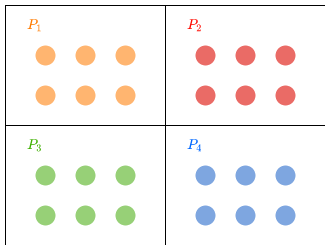
\includegraphics[scale=0.8]{img/STAT4402_tut_KNN_1_no_cap.png}
        \centering
    \end{figure}
    
    \item Determine the closest samples within each process
    \begin{figure}[H]
        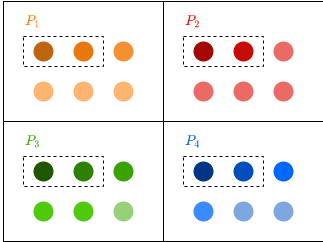
\includegraphics[scale=0.8]{img/STAT4402_tut_KNN_2_no_cap.png}
        \centering
    \end{figure}
    
    \item Collect the \(k^{th}\) closest samples and order them in the master node get the global
\(k^{th}\) closest samples
    \begin{figure}[H]
        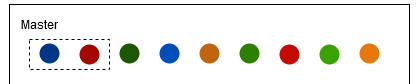
\includegraphics[scale=0.7]{img/STAT4402_tut_KNN_3_no_cap.png}
        \centering
    \end{figure}
\end{enumerate}

\section{Parallel SGD}
As before let $T$ a set of training samples $\left\lbrace \left( \bm{x}_{i}, \bm{y}_i \right) \right\rbrace_{i=1}^{m} = \left\lbrace z_{i} \right\rbrace_{i=1}^{m}$. Let $C \left( \bm{w} \right)$ be the cost function for our model to learn off
\[
    C \left( \bm{w} \right) = \frac{1}{N} \sum_{i=0}^{m} C_{z_{i}}\left( \bm{w} \right).
\]
For gradient descent algorithms, we wish to find a weight vector $\bm{w}^{\ast}$ that minimizes our cost function, that is
\[
    \bm{w}^{\ast} = \underset{\bm{w} \in \mathbb{R}^{n}}{\arg \min } \sum_{i=0}^{m} C_{z_{i}}\left( \bm{w} \right)
\]
For gradient descent algorithms, we wish to find a weight vector $\bm{w}^{\ast}$ that minimizes our cost function, that is
\[
    \bm{w}^{\ast} = \underset{\bm{w} \in \mathbb{R}^{n}}{\arg \min } \sum_{i=0}^{m} C_{z_{i}}\left( \bm{w} \right)
\]
Let's introduce the notation $G \triangleq \frac{\partial C}{\partial \bm{w}}$ and $G_{z} \triangleq \frac{\partial C_{z}}{\partial \bm{w}}$ to simplify gradient notation as well as $H \triangleq \frac{\partial G}{\partial \bm{w}}$ and $H_{z} \triangleq \frac{\partial G_{z}}{\partial \bm{w}}$ to simplify Hessian notation. At each step of the SGD, a sample $z_{j} = \left( \bm{x}_j , y_{j} \right)$ is uniformly selected from the training set to update the existing weight vector as
\[
    \bm{w}_{t+1} = \bm{w}_{t} - \eta_{t} G_{z_{j}} \left( \bm{w}_{t} \right)
\]
where $\eta_{t}$ is just the learning rate at iteration $t$. Say a process performs SGD of a data set $T_{1}$ to get from a weight $\bm{w}_{g}$ to weight $\bm{w}_{1}$. When processing another training set $T_{2}$, a sequential SGD algorithm would have started at weight $\bm{w}_{1}$ to reach a possibly different weight vector $\bm{w}_{h}$. To parallelize the SDG algorithm we wish to start computing of training set $T_2$ on weight vector $\bm{w}_{1}$ while simultaneously running the training set $T_1$ on weight vector $\bm{w}_{g}$, but $\bm{w}_{1}$ is not know until SGD is finished with $T_1$. So how do we get around this? One method is to soundly combine models from different processes in the hopes of achieving a weight vector had the SGD was instead run sequentially \cite{MalekiSaeed2017PSGD}. This requires adjusting the computation of $T_2$ to account for the staleness $\bm{w}_{1} - \bm{w}_{g}$ in the initial model. To do so, the second model performs its computations instead on $\bm{w}_{g} - \Delta \bm{w}$ where $\Delta \bm{w}$ is an unknown symbolic vector. This allows the second model to run in parallel and not have to wait until $\bm{w}_{1}$ is produced from the succeeding model. Once the first process is done, the second process takes $\Delta \bm{w}$ to be $\bm{w}_{1} - \bm{w}_{g}$. This technique can be easily extended to an arbitrary number of processors.\\[1\baselineskip]
Let $S_{T} \left( \bm{w} \right)$ represent the SGD computation of a training $T$ from an initial weight vector $\bm{w}$, for example $S_{T_{1}} \left( \bm{w}_{g} \right) = \bm{w}_{1}$. To come up with a model combiner we need to think about how we can calculate
\[
    S_{T} \left( \bm{w} + \Delta \bm{w} \right).
\]
Assuming $S_{T}$ is differentiable at $\bm{w} + \Delta \bm{w}$, we get the following by consider the Taylor series of $S_{T}$ about the point $\bm{w} + \Delta \bm{w}$
\[
    S_{T} \left( \bm{w} + \Delta \bm{w} \right) = S_{T} \left( \bm{w} \right) + S_{T} ' \left( \bm{w} \right) \cdot \Delta \bm{w} + \mathcal{O} \left( \left| \Delta \bm{w} \right|^{2} \right).
\]
We will introduce the notation $M_{D} \triangleq S_{T}'$ as the model combiner. In the equation above the model combiner captures the first order information of how a change in $\Delta \bm{w}$ will effect the SGD. When $\Delta \bm{w}$ is sufficiently small, one can neglect higher order terms and only use the model combiner to combine models from different processes. From \cite{MalekiSaeed2017PSGD} we can show that for a sequence of input examples $z_1 , z_2, \ldots , z_{n}$ the model combiner can be computed as
\[
    M_{D} (\bm{w}) = \prod_{i=1}^{n} \left( \bm{I} - \eta_{i} \cdot H_{z_{i}} \left( S_{T_{i-1}} \left( \bm{w} \right) \right) \right)
\]
where $S_{T_{0}} \left( \bm{w} \right) = \bm{w}$. This result can be easily shown by applying the chain rule to $S_{T} \left( \bm{w} \right) = S_{T_{n}} \left( S_{T_{n-1}} \left( \ldots \left( S_{1} \left( \bm{w} \right) \right) \right) \right)$. We will introduce the notation $M_{D} \triangleq S_{T}'$ as the model combiner. In the equation above the model combiner captures the first order information of how a change in $\Delta \bm{w}$ will effect the SGD. When $\Delta \bm{w}$ is sufficiently small, one can neglect higher order terms and only use the model combiner to combine models from different processes. From \cite{MalekiSaeed2017PSGD} we can show that for a sequence of input examples $z_1 , z_2, \ldots , z_{n}$ the model combiner can be computed as
\[
    M_{D} (\bm{w}) = \prod_{i=1}^{n} \left( \bm{I} - \eta_{i} \cdot H_{z_{i}} \left( S_{T_{i-1}} \left( \bm{w} \right) \right) \right)
\]
where $S_{T_{0}} \left( \bm{w} \right) = \bm{w}$. This result can be easily shown by applying the chain rule to $S_{T} \left( \bm{w} \right) = S_{T_{n}} \left( S_{T_{n-1}} \left( \ldots \left( S_{1} \left( \bm{w} \right) \right) \right) \right)$.\\[1\baselineskip]
Thus to create a parallelized SGD, each of the $p$ processors start with the same initial global weight vector $\bm{w}_{g}$ to compute its local model $S_{T_i} \left( \bm{w}_{g} \right)$ and model combiner $M_{T_{i}} \left( \bm{w}_{g} \right)$ in parallel. A subsequent reduction phase computes $\bm{w}_{i}$ by adjusting the input of processor $i$ by adjusting by the staleness introduced in the $i-1$ processor
\[
    \bm{w}_{i} = S_{T_{i}} \left( \bm{w_{g}} \right) + M_{T_{i}} \left( \bm{w}_{g} \right) \cdot \left( \bm{w}_{i-1} - \bm{w}_{g} \right).
\]
The algorithm for parallel SGD is summarised in algorithm \ref{alg:parallel-SGD}

\begin{algorithm}[ht!!!]
    \caption{Parallel SGD}
    \label{alg:parallel-SGD}
    \SetAlgoLined
    \SetKwInOut{Input}{input}\SetKwInOut{Output}{output}
    \Input{Training data $T$, an initial weight vector $\bm{w}_{g}$ and the number of processes to perform the algorithm $p$}
    \Output{Updated weight vector}
    \BlankLine
    $\left\lbrace T_{1} , T_{2}, \ldots , T_{p} \right\rbrace \gets$ an equal partition of $T$\;
    \For{$T_{i} \in \left\lbrace T_{1} , T_{2}, \ldots , T_{p} \right\rbrace$ {\bf concurrently}}{
        Compute $S_{T_{i}} \left( \bm{w_{g}} \right)$ and $M_{T_{i}} \left( \bm{w}_{g} \right)$\;
    }
    \For{$i \in \left\lbrace 1,2, \ldots , p \right\rbrace$}{
        $\bm{w}_{i} \gets S_{T_{i}} \left( \bm{w_{g}} \right) + M_{T_{i}} \left( \bm{w}_{g} \right) \cdot \left( \bm{w}_{i-1} - \bm{w}_{g} \right)$\;
    }
    \KwResult{$\bm{w}_{p}$}
    \BlankLine
\end{algorithm}

% SGD theory

% Log onto HPC w/ examples

% Questions

% Answers

% References

%% References without bibTeX database:

\bibliographystyle{model1-num-names}
\bibliography{bib_ref}

\end{document}